\subsection{Logistic Regression Model}
A summary of the f1-scores and accuracies produced by the different Logistic Regression Model variations can be observed in figure \ref{LR-model-scores-table}. 
As shown, the DistilBERT model outperforms both the Word2Vec and TF-IDF models by obtaining higher evaluation metrics, whereas the TF-IDF performs the worst. 
Additionally, in figure \ref{LR-model-confusion-matrices}, one may observe how well each model predicted the genre of a movie for each class. 
It can first be noted that the DistilBERT model (on the far right) has the brightest (most yellow) diagonal indicating that it had the greatest number of correct classifications. 
Additionally, labels 0, 4, and 7 have the greatest amount of data likely representing the most common genres in the dataset (Action, Comedy, and Drama). 
Furthermore, considering the diagonal is brightest for those three genres across all models, this clearly represents that the models are best at predicting these genres, as they are represented the greatest in the dataset. 
On the other hand, labels such as 8 (Fantasy), 9 (Film-Noir), 11 (IMAX), 12 (Musical), 13 (Mystery), and 14 (Romance) have no predictions across all the models, likely indicating these are under-represented genres in the dataset. 
This further supports that the model is bad at classifying these genres since, as mentioned previously, they are under-represented in the dataset. 
Additionally, a pattern in the error is that all the models mis-classify rare genres into the more common ones. 
For example, predicting crime (5) as comedy (4). 
This incorrect pattern may be fixed by, collecting more data for the under-represented genres, augmenting the data, or using a weighted loss function. 

\begin{figure*}[t]
  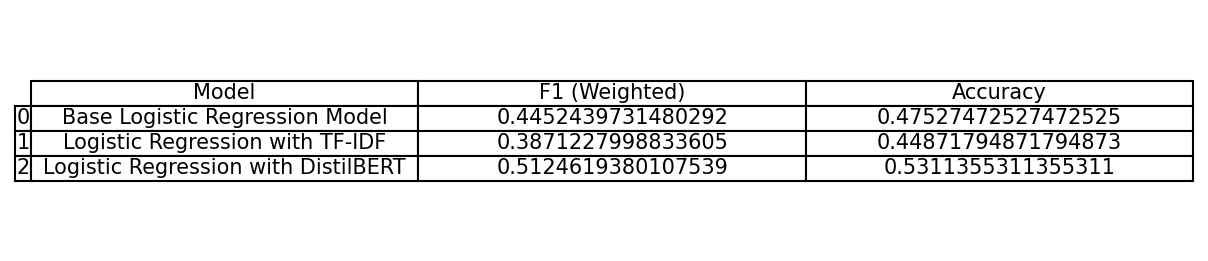
\includegraphics[width=\linewidth]{Nour/Images/model-scores.png} \hfill
  \caption {Comparison of the f1-scores and accuracies of the different Logistic Regression Model variations.}
  \label{LR-model-scores-table}
\end{figure*}

\begin{figure*}[t]
  
\includegraphics[width=\linewidth]{Nour/Images/confusion_matrices.png} \hfill
  \caption {Confusion matrices for the different Logistic Regression Model variations.}
  \label{LR-model-confusion-matrices}
\end{figure*}